%!TEX root = ../Project.tex

\subsection{Database structure}
\label{developmentdatabasestructure}

As relational databases are so popular and are supported in many software
frameworks, there is no advantage to choosing a database model other than
relational. Web frameworks abstract away any code related to a specific
database product using an \gls{orm}, so the module allocation application can
be written without regard for the final database product that \gls{itservices}
will use to deploy the application.

Preliminary conversations with departmental administrators informed the
database structure. Firstly, there are several entities stored by the
University that will be useful to this system, which have the properties given
in Table~\ref{development_database_uni_entities}.

\begin{table}
  \begin{center}
    \begin{tabular}{ | l | l | }
      \hline
      \textbf{Entity} & \textbf{Properties} \\
      \hline
      Student    & Username (unique), \gls{routecode}, \gls{stage} \\
      Module     & Module code (unique), module name, number of credits, maximum class size \\
      \hline
    \end{tabular}    
  \end{center}
  \caption{Entities and their properties as stored by the University of York}
  \label{development_database_uni_entities}
\end{table}

Each module is given a number of credits representing the estimated workload
for that module, and each student must take 120 credits every academic year.

The two pilot departments currently use paper forms, some of which are given
in Appendix~\ref{sec:paperforms}. In order to create a scalable system that
could be used across any number of departments, I first generalised the paper
forms provided by the pilot departments. This generalisation involved the
following observations:

\begin{itemize}
  \item Each degree type (single subject, joint honours, etc) can receive a different form
  \item Each form contains one or more groups, and each group contains one or more modules
  \item A student will be allocated a certain number of modules from each group
\end{itemize}

These observations led to the creation of a database structure given in
Table~\ref{development_database_schema}. Primary keys are
\underline{underlined}, foreign keys are \emph{in italics}. If no primary key
is given for an entity, an automatically incrementing integer is used.

\begin{table}
  \begin{center}
    \begin{tabular}{ | l | l | }
      \hline
      \textbf{Entity} & \textbf{Properties} \\
      \hline
      Sheet & \underline{\gls{routecode}}, \underline{\gls{stage}}, student help \\
      Group & \emph{Sheet}, title, student help, credits to allocate \\
      Module & \underline{module code}, module name, \emph{Department} \\
      Module Availability & \emph{Module}, credits, student min, student cap \\
      Student & \underline{username}, date ranked, \emph{Sheet}, \emph{Department} \\
      Elective & \emph{Student}, \emph{Group}, credits \\
      Department & name \\
      Staff & \underline{username}, \emph{Department} \\
      Allocation & \emph{Student}, \emph{Module Availability} \\
      Choice & \emph{Student}, \emph{Module Availability}, rank \\
      \hline
    \end{tabular}
  \end{center}
  \caption{Entities stored in the module allocation application}
  \label{development_database_schema}
\end{table}

As one would expect, a sheet entity is a replacement for the current paper
sheets used by departments. It is unique by type of student (\gls{routecode})
and by their year of study. A sheet can contain one or more group entities.
There is a many-to-many relationship between groups and module availabilities.
A module availability is an instance of a module in a specific term or year.

Every student is assigned to a specific sheet, which informs the groups and
modules that are available to them. Every choice the student makes is stored
in the database along with the rank they gave that module, and an allocation
is simply a student, module pair.

% [@todo what normal form is this in?]

\subsubsection{Entity-relationship diagram}

Figure~\ref{er_diagram} is an entity-relationship diagram of the module
allocation system.

\begin{landscape}
  \begin{figure}
    \centering
    \fbox{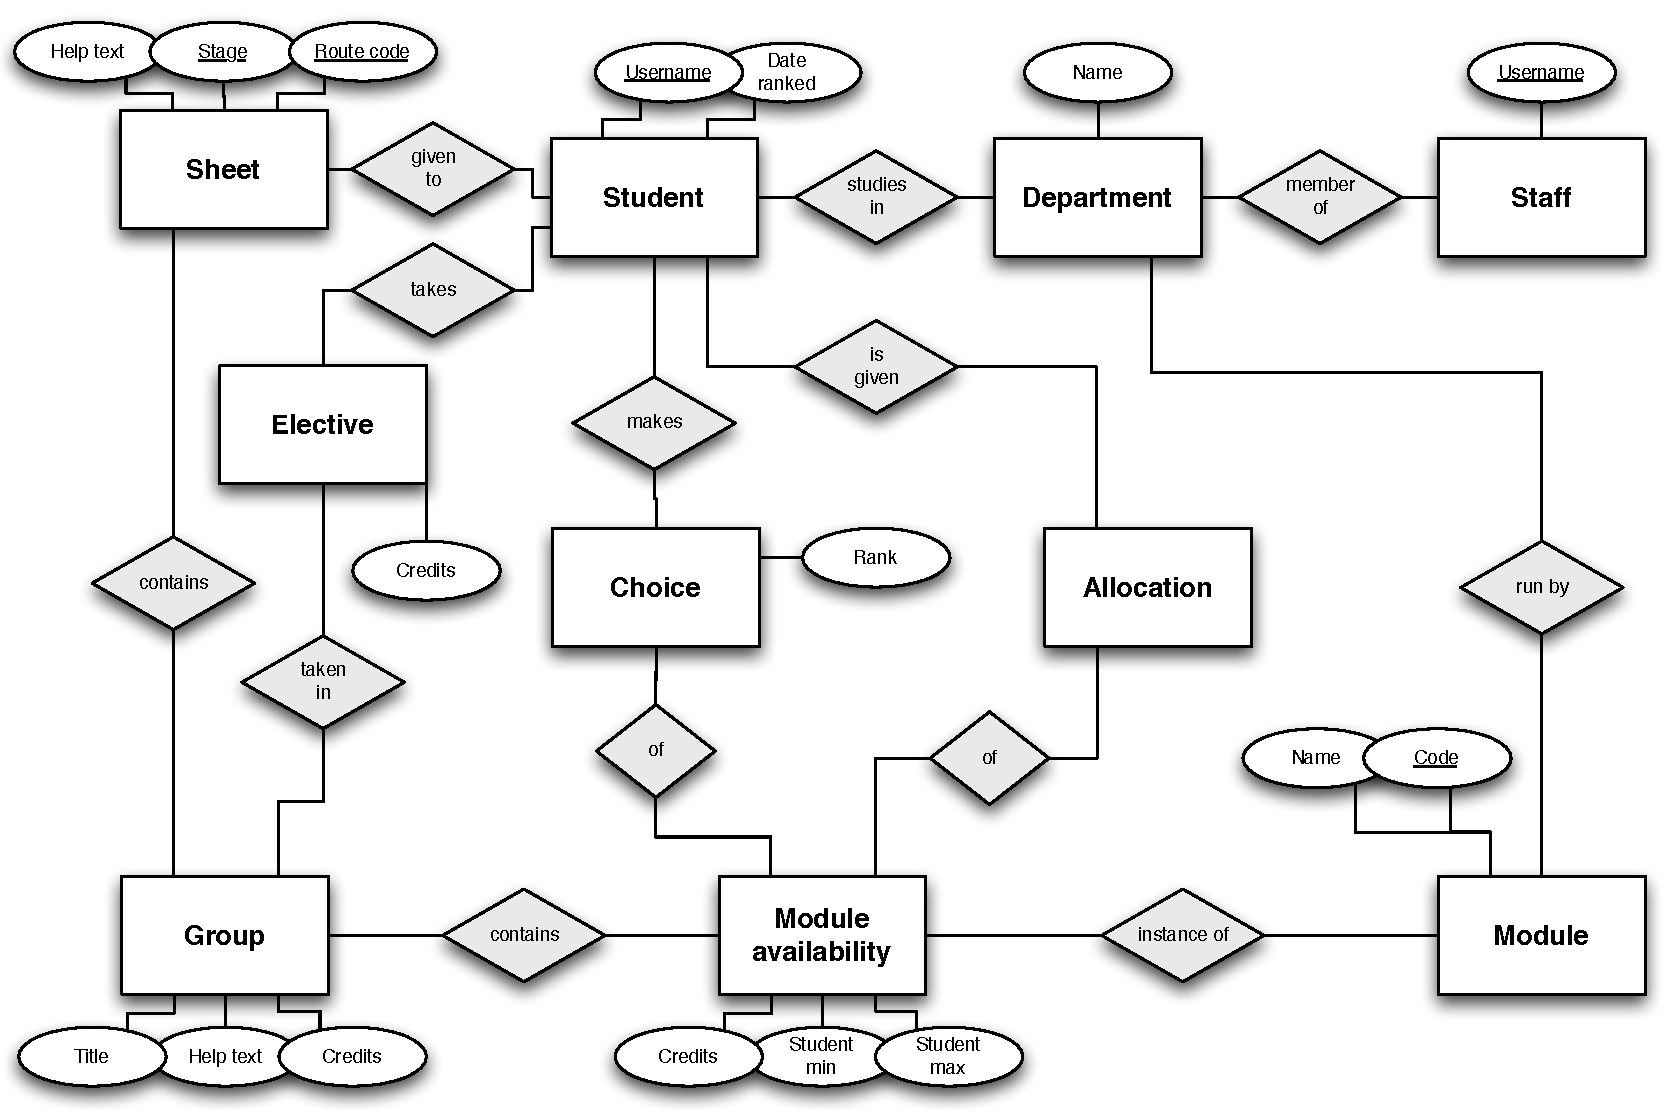
\includegraphics[width=0.9\linewidth]{inc/er_diagram.pdf}}
    \caption{Entity-relationship diagram for the module allocation system}
    \label{er_diagram}
  \end{figure}
\end{landscape}
